% Options for packages loaded elsewhere
\PassOptionsToPackage{unicode}{hyperref}
\PassOptionsToPackage{hyphens}{url}
%
\documentclass[
  12pt,
]{article}
\usepackage{lmodern}
\usepackage{amssymb,amsmath}
\usepackage{ifxetex,ifluatex}
\ifnum 0\ifxetex 1\fi\ifluatex 1\fi=0 % if pdftex
  \usepackage[T1]{fontenc}
  \usepackage[utf8]{inputenc}
  \usepackage{textcomp} % provide euro and other symbols
\else % if luatex or xetex
  \usepackage{unicode-math}
  \defaultfontfeatures{Scale=MatchLowercase}
  \defaultfontfeatures[\rmfamily]{Ligatures=TeX,Scale=1}
\fi
% Use upquote if available, for straight quotes in verbatim environments
\IfFileExists{upquote.sty}{\usepackage{upquote}}{}
\IfFileExists{microtype.sty}{% use microtype if available
  \usepackage[]{microtype}
  \UseMicrotypeSet[protrusion]{basicmath} % disable protrusion for tt fonts
}{}
\usepackage{xcolor}
\IfFileExists{xurl.sty}{\usepackage{xurl}}{} % add URL line breaks if available
\IfFileExists{bookmark.sty}{\usepackage{bookmark}}{\usepackage{hyperref}}
\hypersetup{
  pdftitle={Spotify Clarifies},
  pdfauthor={Britney Brown, Harrison DiStefano, Greg Eastman; Lisa Kaunitz, Tianyang Liu, Jeremy Weidner},
  hidelinks,
  pdfcreator={LaTeX via pandoc}}
\urlstyle{same} % disable monospaced font for URLs
\usepackage[left=12mm, right=12mm, top=15mm, bottom=15mm]{geometry}
\usepackage{graphicx}
\makeatletter
\def\maxwidth{\ifdim\Gin@nat@width>\linewidth\linewidth\else\Gin@nat@width\fi}
\def\maxheight{\ifdim\Gin@nat@height>\textheight\textheight\else\Gin@nat@height\fi}
\makeatother
% Scale images if necessary, so that they will not overflow the page
% margins by default, and it is still possible to overwrite the defaults
% using explicit options in \includegraphics[width, height, ...]{}
\setkeys{Gin}{width=\maxwidth,height=\maxheight,keepaspectratio}
% Set default figure placement to htbp
\makeatletter
\def\fps@figure{htbp}
\makeatother
\setlength{\emergencystretch}{3em} % prevent overfull lines
\providecommand{\tightlist}{%
  \setlength{\itemsep}{0pt}\setlength{\parskip}{0pt}}
\setcounter{secnumdepth}{-\maxdimen} % remove section numbering
\usepackage{indentfirst} \usepackage{background} \usepackage{float} \backgroundsetup{ scale=1, color=black, angle=0, pages=all, contents={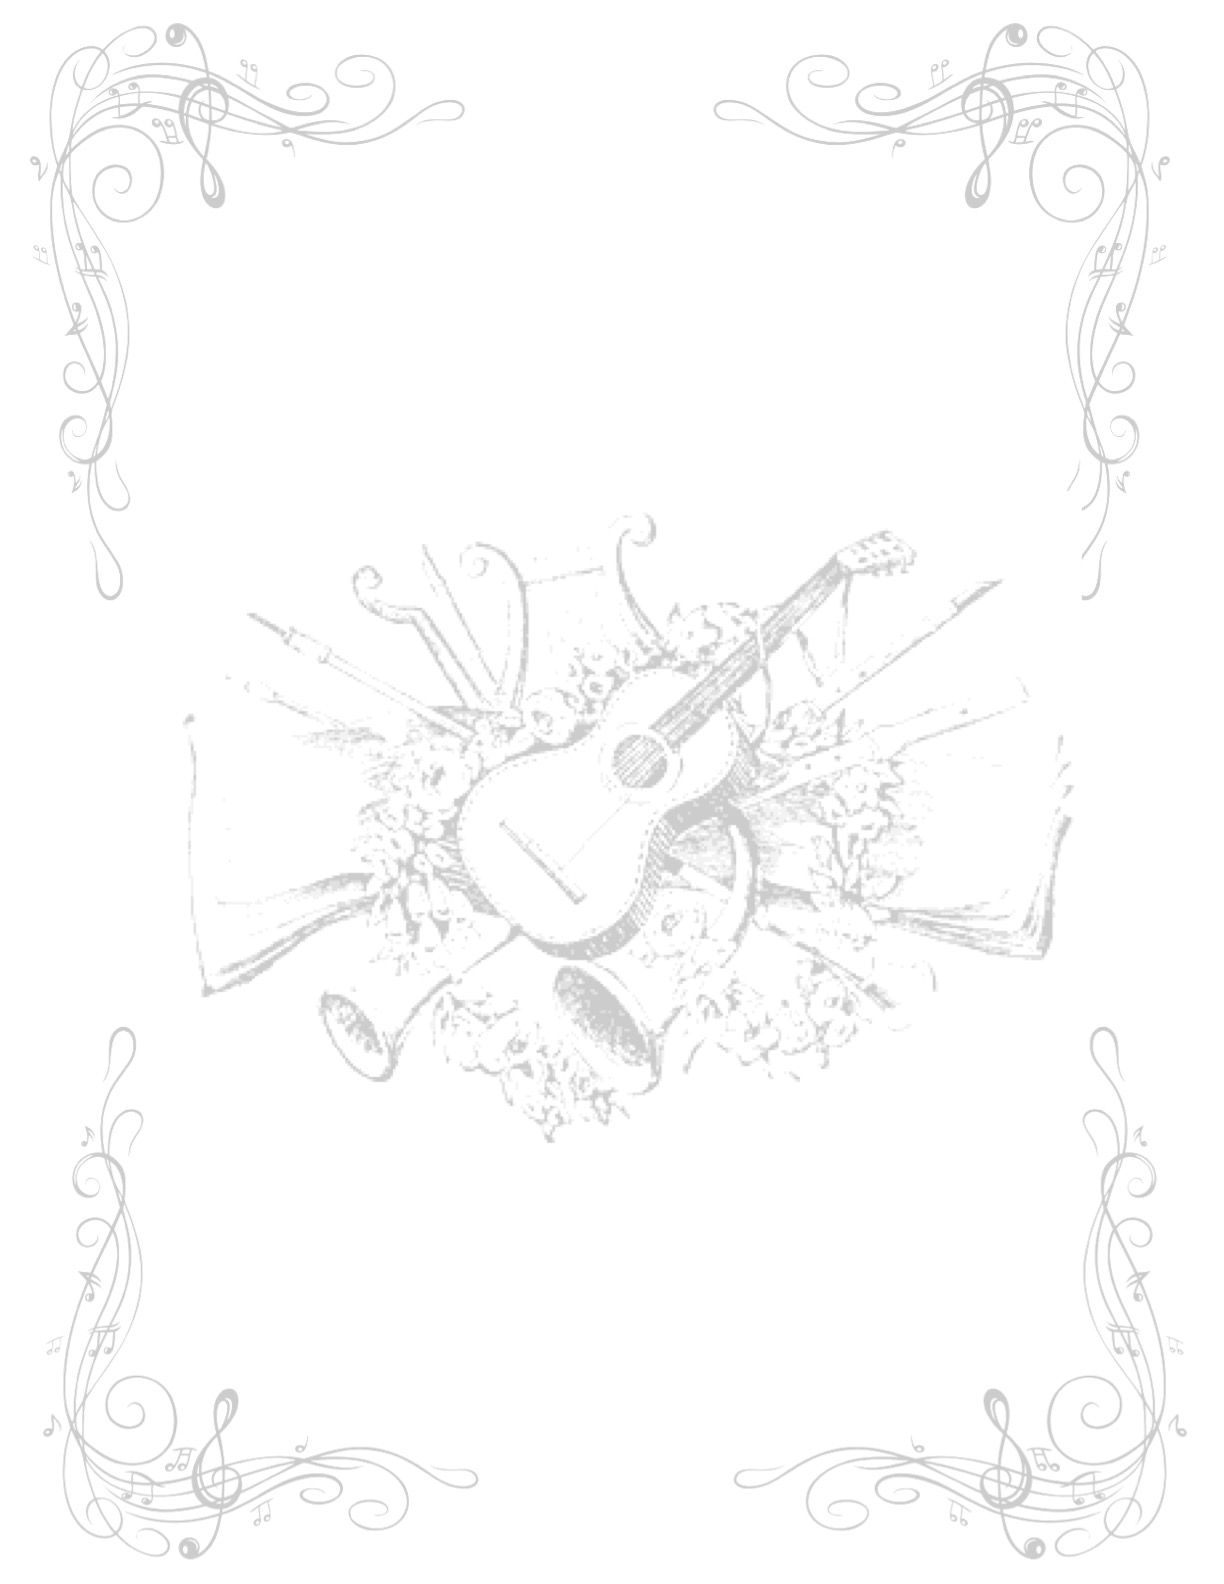
\includegraphics[width=22cm,height=52cm]{music_graphic.jpg}} }
\usepackage{booktabs}
\usepackage{longtable}
\usepackage{array}
\usepackage{multirow}
\usepackage{wrapfig}
\usepackage{float}
\usepackage{colortbl}
\usepackage{pdflscape}
\usepackage{tabu}
\usepackage{threeparttable}
\usepackage{threeparttablex}
\usepackage[normalem]{ulem}
\usepackage{makecell}
\usepackage{xcolor}

\title{Spotify Clarifies}
\usepackage{etoolbox}
\makeatletter
\providecommand{\subtitle}[1]{% add subtitle to \maketitle
  \apptocmd{\@title}{\par {\large #1 \par}}{}{}
}
\makeatother
\subtitle{An Analysis of Music Popularity over Time}
\author{Britney Brown, Harrison DiStefano, Greg Eastman \and Lisa
Kaunitz, Tianyang Liu, Jeremy Weidner}
\date{06/09/2021}

\begin{document}
\maketitle

\vspace{8pt}

Music has been an integral part of our culture since well before the
invention of the computer. Lately we have seen digital music take the
industry by storm, which for the first time in musical history gives us
the ability to analyze the quantifiable components of the music we all
enjoy. Popular music has evolved significantly over the last fifty years
from songs like the Beatles' ``I Want to Hold Your Hand'' to Taylor
Swift's ``Shake it Off.'' Although we recognize a shift here, what can
the data behind these songs tell us about trends in the music industry?

\vspace{12pt}

\hypertarget{key-insights}{%
\subsection{Key Insights}\label{key-insights}}

Through our analysis of musical attributes, we found four interesting
results:

\begin{itemize}
\item
  We discovered two important themes that span across all time: emotions
  and relationships. Regardless of societal evolution, the want to
  express our emotions towards the people we care for is a constant
  force.
\item
  We also found that people tend to prefer sad, depressing songs more in
  the recent years due to a decrease in valence (positive sounds) and
  increase in minor modes. A quick scan of current events probably makes
  this one of our less surprising findings.
\item
  In order for a song to be considered ``danceable'', there should be
  some acoustic presence, high valence, a slightly above average
  loudness, and an avoidencess of too much instrumentalness.
\item
  In the last 20 years, tracks have consistently maintained
  approximately nine sections. This steady approach to song structure
  highly suggests the introduction of a breakthrough algorithmic
  approach towards song creation in order to increase success potential.
\end{itemize}

\newpage

\hypertarget{song-titles}{%
\subsection{Song Titles}\label{song-titles}}

A text mining analysis of song titles revealed the importance of the
term ``love''. This lead us to explore the prevalence of emotions in
song titles as well as the people mentioned, such as ``baby,'' ``boy,''
and ``girl''. These descriptions of who these people are to the artists
of each song revealed that regardless of time, music will forever be
used to express our feelings towards the people that mean the most to
us.

\vspace{4pt}

\hypertarget{musical-attributes}{%
\subsection{Musical Attributes}\label{musical-attributes}}

Using data from Spotify's Web API, we analyzed song construction to
better understand what makes particular songs timeless and others
forgettable. We looked at the overall trends in music theory variables
such as tempo, time signature, and key signature as well as attributes
defined by Spotify such as danceability, acousticness, loudness,
instrumentalness, and valence. These results revealed patterns that were
constant in hit tracks over the span of six decades as well as those
that indicate a change in our listening preferences over time. We dove
even further into our analysis through the decades by comparing song
duration and major and minor mode percentages, further verifying our
results in the evolution of music preference.

\begin{center}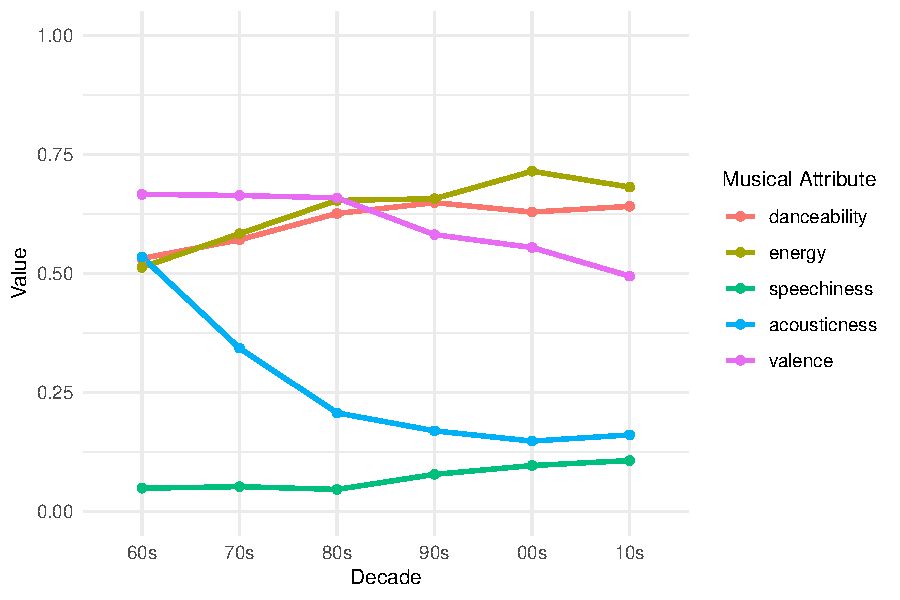
\includegraphics{Final_summary_405_majestic_capybara_files/figure-latex/unnamed-chunk-1-1} \end{center}

\hypertarget{track-production}{%
\subsection{Track Production}\label{track-production}}

Finally, our goal to achieve a better interpretation of musical trends
was not only achieved, but we also gained a greater understanding of the
modern music world. A visual exploration of our section variables
revealed that in the last 20 years, tracks have consistently maintained
approximately nine sections including intro, verse 1, pre-chorus,
chorus, verse 2, pre-chorus, chorus, bridge, and outro. We believe this
indicates the introduction of a formulaic or even algorithmic approach
to producing songs in recent years. Our analysis indicates a more
constant, rigid structure in hit songs that the music industry utilizes
to increase a track's potential to become a hit. A query of top artists
over the years verified this intuition by demonstrating a shift in song
production over the decades: artists in the 60s and 70s had a focus on
larger outputs of songs while current arists are more focused on the
quality of the songs shared with the public.

\end{document}
